\chapter{Conclusioni}

Il nostro obiettivo principale è quello di applicare un modello di Data Coverage facilmente replicabile a vari scenari di Mobile Crowdsensing e, contemporaneamente, di sviluppare una strategia efficace per l'arricchimento sintentico dei dataset di mobilità disponibili pubblicamente.
Librerie versatili e complete come scikit-mobility \cite{pappalardo2019scikitmobility} ci hanno aiutato a svolgere compiti affatto banali e a ottenere metriche utili sul nostro dataset. I tool grafici poi, ci hanno permesso di rappresentare risultati di Data Coverage ottenuti grazie al modello descritto nel Capitolo 2 in modo chiaro e diretto.
Grazie a tali librerie, e agli strumenti esplorativi della Data Science, siamo riusciti nel nostro intento di modellare la Data Coverage e di calcolarla sul dataset arricchito, producendo così delle mappe probabilistiche di Coverage che possano essere utilizzate in lavori futuri.
L'implementazione del modello e la sua successiva applicazione a scenari diversi per finalità e composizione è, a nostro avviso, il risultato più interessante di questa tesi.
Ci riteniamo soddisfatti dei risultati che abbiamo raggiunto in questi ambiti, tuttavia ci sono alcuni aspetti del nostro studio che potrebbero essere ampliati e approfonditi in futuro; grazie alla Data Coverage che abbiamo calcolato, infatti, è possibile pianificare uno sviluppo del lavoro che sia guidato da tale metrica.
Vorremmo di seguito descrivere brevemente tre dei possibili sviluppi in questo senso.

\paragraph*{Utilizzo della Data Coverage per il posizionamento di UAV Base Stations}
Grazie alla Data Coverage calcolata, sarà possibile scegliere il posizionamento ottimale per una o più stazioni di ricarica per UAV (unmanned aerial vehicles). Queste stazioni fungeranno da punti di partenza e arrivo per droni a pilotaggio remoto (possibilmente automatico, e schedulato sulla base della evoluzione dinamica della data coverage nella area di sensing) che sorvolino le aree con una Data Coverage pessima o inesistente, al fine di raccogliere loro stessi i dati mancanti.
Tale attività rappresenta la naturale
continuazione di questo lavoro di tesi su cui altri studenti potranno condurre ulteriori attività di ricerca.
Le immagini presenti in Figura \ref{fig:uav_stations} mostrano un possibile posizionamento per le stazioni di ricarica.

\begin{figure}
	\centering
	\begin{subfigure}[b]{\linewidth}
		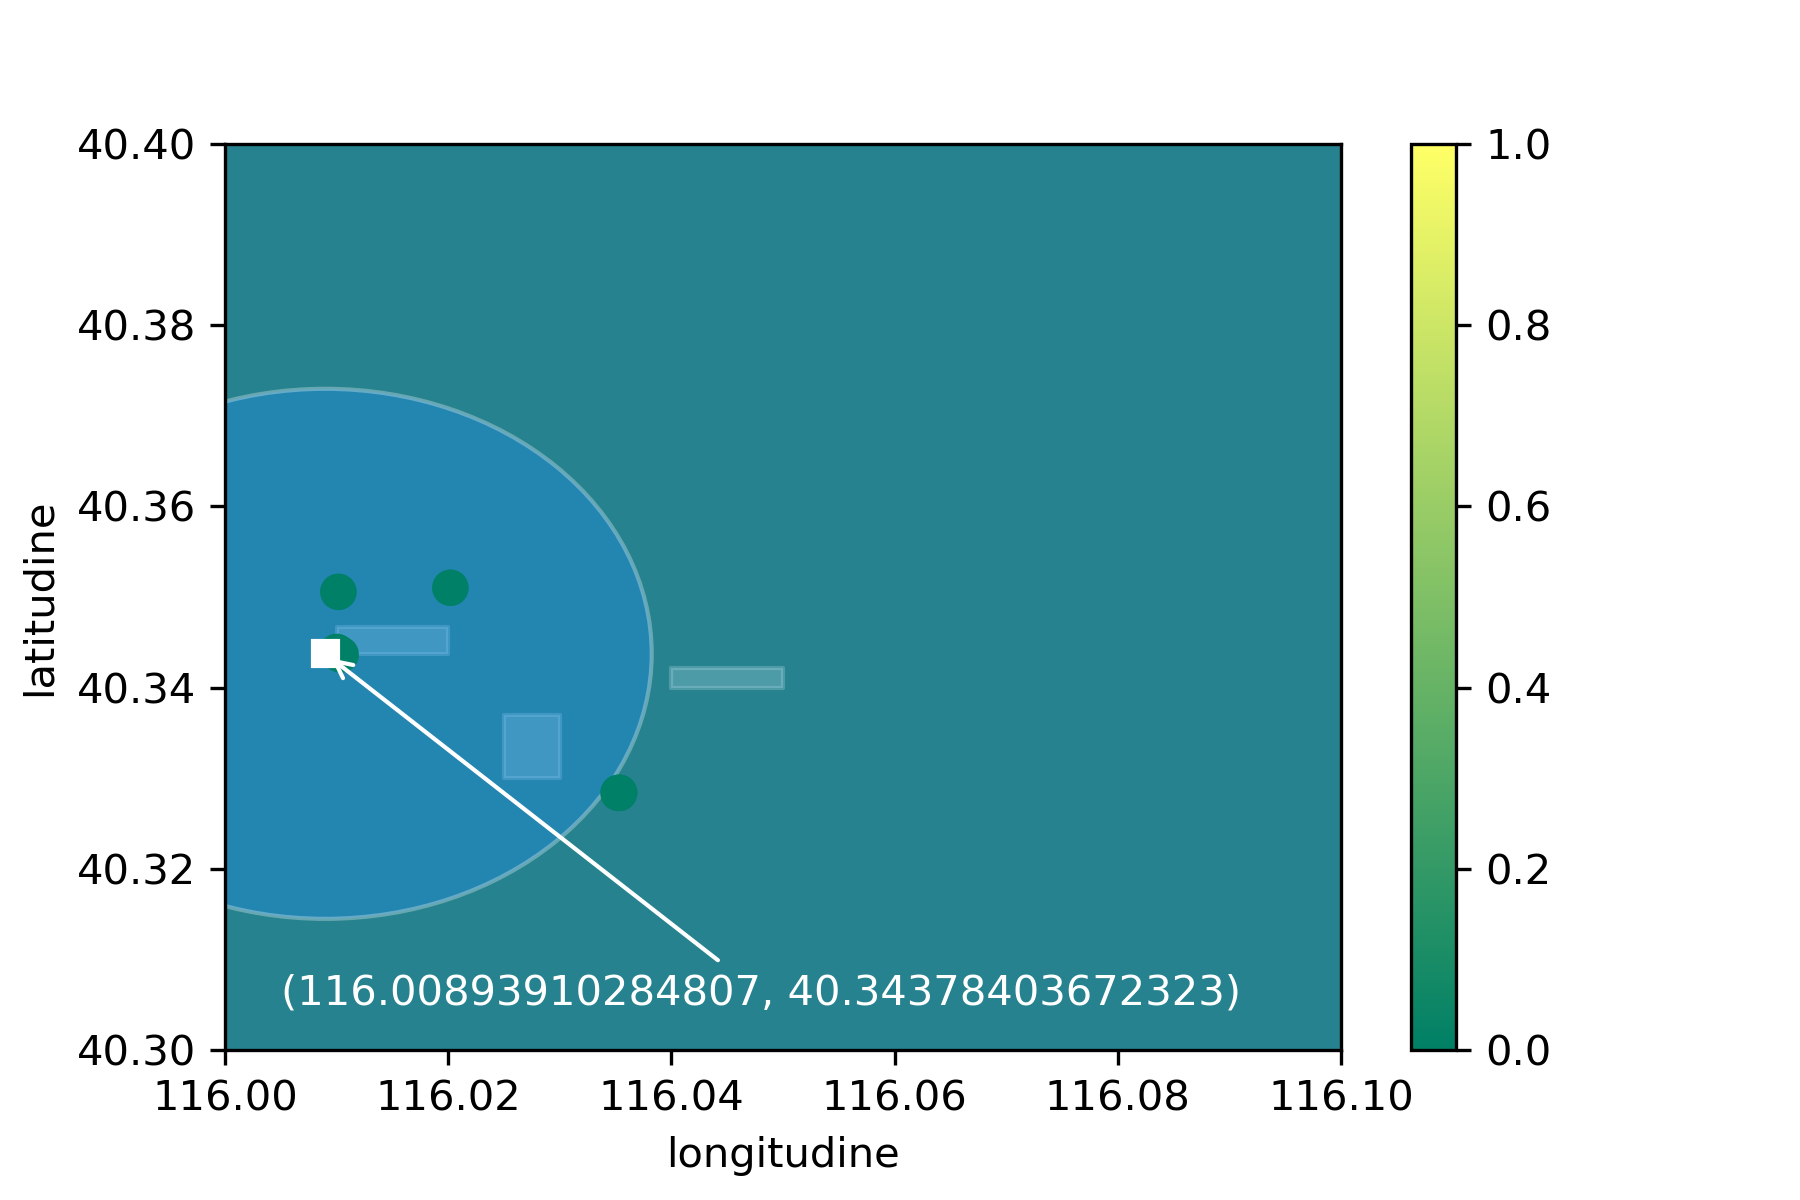
\includegraphics[width=\linewidth]{drone_low_cov_squares.png}
		\caption{Posizionamento su mappa con cattiva Data Coverage. I rettangoli chiari rappresentano zone in cui non è possibile posizionare la stazione di ricarica.}
	\end{subfigure}
	\begin{subfigure}[b]{\linewidth}
		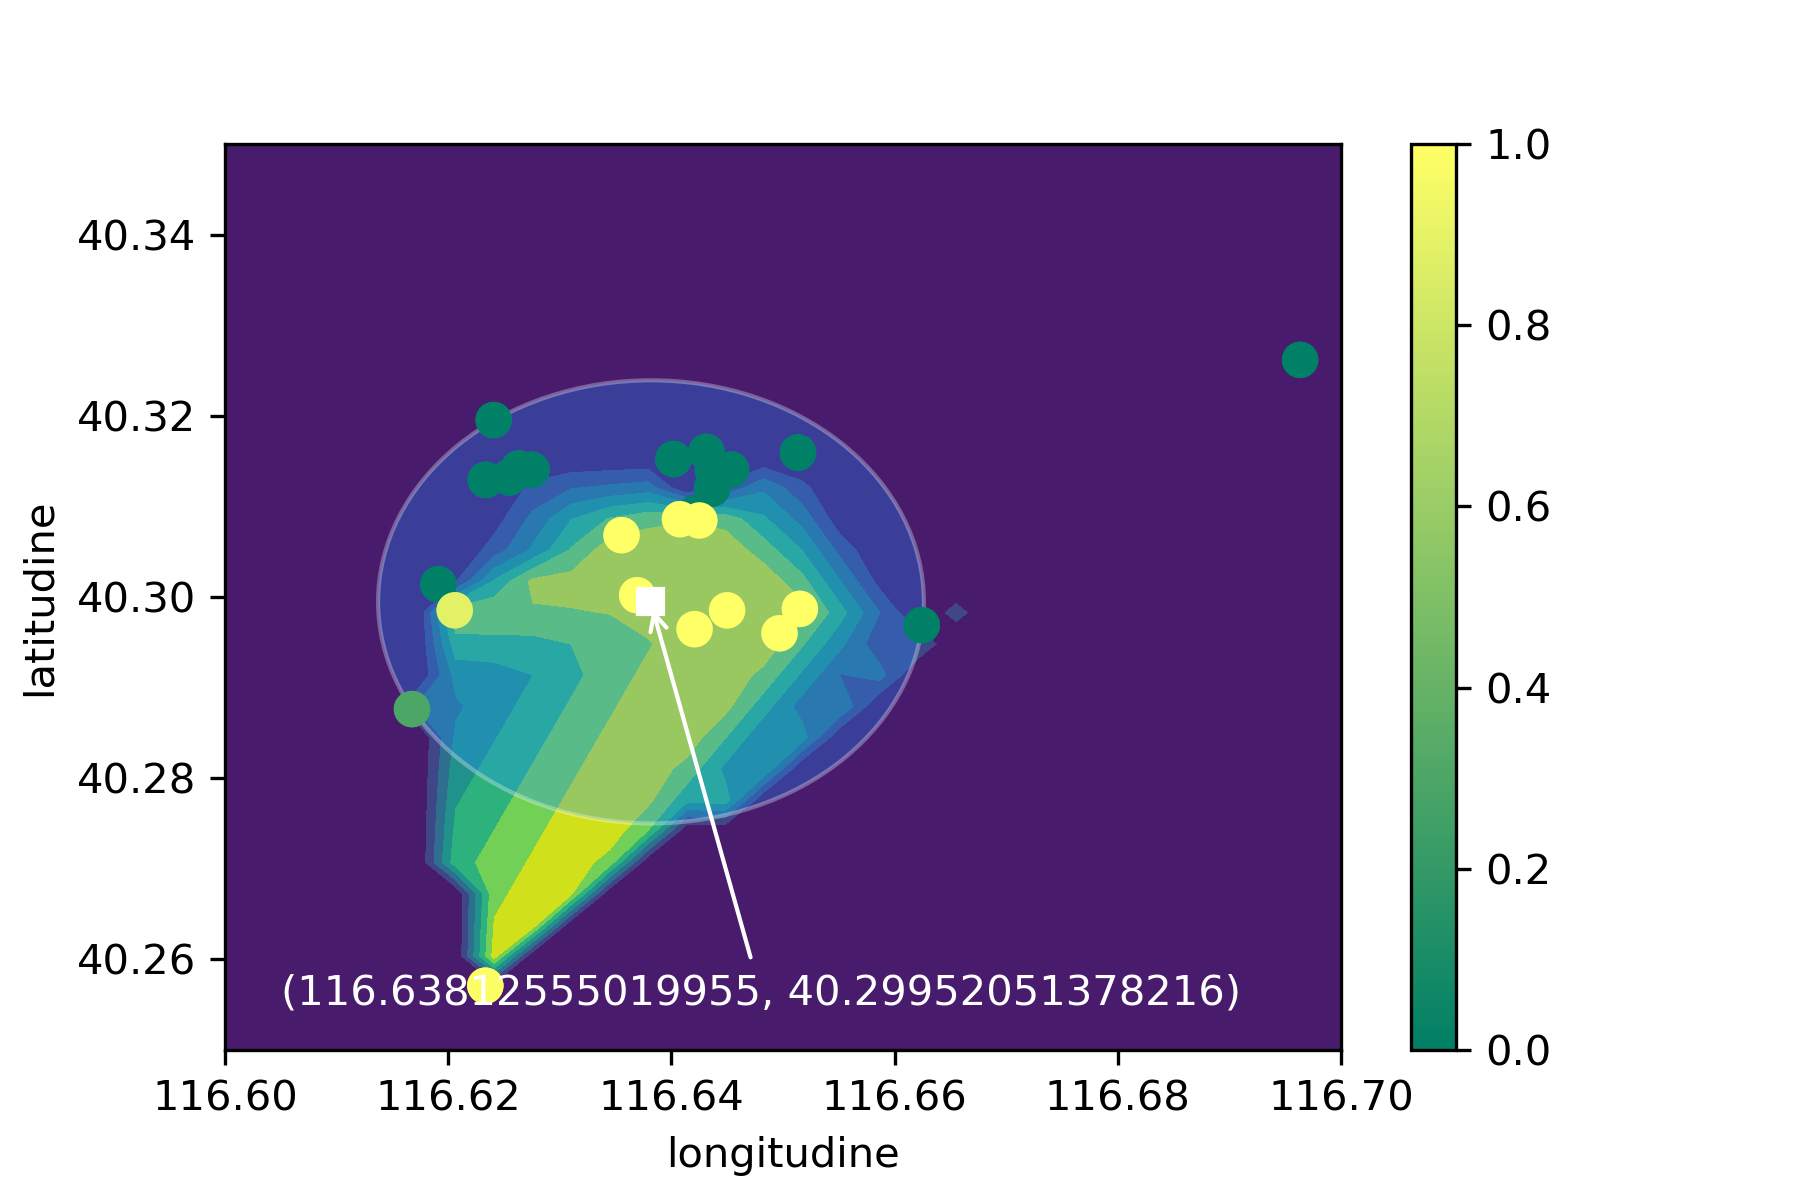
\includegraphics[width=\linewidth]{drone_med_cov.png}
		\caption{Posizionamento su mappa con Data Coverage accettabile.}
	\end{subfigure}
	\caption[Posizionamento di UAV Base Stations]{Esempi di posizionamento di una stazione di ricarica per UAV su una mappa di Data Coverage. I quadrati bianchi rappresentano la posizione della stazione di ricarica, il cerchio attorno ad essi rappresenta il raggio della zona coperta dal drone.}
	\label{fig:uav_stations}
\end{figure}

\paragraph{Calcolo della Coverage a partire dalla mobilità degli utenti tramite strumenti predittivi}
Partendo dalle traiettorie note degli utenti, è possibile sviluppare strumenti predittivi che utilizzino metriche quali la frequenza e la periodicità degli spostamenti dei singoli individui al fine di predirne il posizionamento futuro. Questo permetterebbe lo sviluppo di modelli di Data Coverage predittivi, utili nella pianificazione di campagne di MCS continuative e dinamiche, che sfruttino queste metriche per ottimizzare l'allocazione di risorse umane a materiali in relazione alle necessità future. 

\paragraph{Uso della Data Coverage per ottimizzare la progettazione di architetture di MCS adattive alla mobilità ed alla quantità di dati}
Questo punto si collega strettamente ai due precedenti. La possibilità di predire la Data Coverage futura, assieme alla versatilità dei droni, sono strumenti utili alla progettazione di architetture MCS il più possibile adattive e dinamiche. Nel recente passato, ad esempio, le nostre abitudini giornaliere sono cambiate molto a causa della pandemia di Covid-19 \cite{DiRenzo2020}: le persone tendono a muoversi meno e a evitare assembramenti, riducendo al tempo stesso l'utilizzo di trasporto pubblico. Date queste premesse, è senz'altro interessante teorizzare e sviluppare architetture MCS resilienti a questo tipo di modificazioni strutturali nel comportamento umano.